\documentclass[11pt]{article} 

% packages with special commands
\usepackage{amssymb, amsmath}
\usepackage{epsfig}
\usepackage{array}
\usepackage{ifthen}
\usepackage{color}
\usepackage{fancyhdr}
\usepackage{graphicx}
%\usepackage{mathtools}
\definecolor{grey}{rgb}{0.5,0.5,0.5}

\begin{document}
\newcommand{\tr}{\text{tr}}
\newcommand{\E}{\textbf{E}}
\newcommand{\diag}{\text{diag}}
\newcommand{\argmax}{\text{argmax}}
\newcommand{\argmin}{\text{argmin}}
\newcommand{\Cov}{\text{Cov}}
\newcommand{\Vol}{\text{Vol}}
\pagestyle{fancy}

\title{A principled approach to decoding}

\author{Charles Zheng and Yuval Benjamini}

\maketitle

\begin{abstract}
The goal of these function MRI studies is to understand the
relationship between $x^{(t)}$ and $y^{(t)}$, where $x^{(t)}$ is a
vector of stimuli features and $y^{(t)}$ is a vector of brain activity
features: this goal can be subdivided into the subgoal of learning an
\emph{encoding model}, which predicts the response $y$ given the
simulus, and the subgoal of learning a \emph{decoding model}, which
reconstructs the stimulus given the response $y$.  One could interpret
both models as multivariate regression problems, with encoding fitting
a model of the form $Y = f(X) + \epsilon$ and decoding fitting a model
of the form $X = g(Y) + \varepsilon$.  However, the regression
formulation is not the only interpretation of the encoding/decoding
problem.  Notably, Kay \emph{et al} treat the encoding problem as a
linear model, but pose the decoding problem as one of
\emph{identification}: that is, given stimuli-response pairs
$(x^{[i_1]}, y^{(1)}), \hdots, (x^{[i_j]}, y^{(j)})$ where the
unobserved $x^{[i]}$ lie in a known set of stimuli $S =
\{x^{[1]},\hdots, x^{[|S|]}\}$, correctly recover the labels
$i_1,\hdots, i_j$ given only the responses $y^{(1)}, \hdots, y^{(j)}$.
Furthermore, Kay \emph{et al} quantify the quality of the decoding
model by the classification rate for the identification problem when
$S$ is selected randomly from a larger database of images
$\mathcal{S}$ (Kay 2008, Vu 2011).  This approach is more suited for
the goal of identifying \emph{natural images} from fMRI responses, and
has been adopted by numerous fMRI studies (Chen 2013). Such studies
usually use a combination of multivariate linear or nonlinear models
and feature selection to implement the decoding model.  However, such
studies have not explicitly motivated their decoding models based on
the criterion of maxmizing correct classification for random stimuli
subsets.  We proposed a principled approach to decoding, wherein we
formulate a decoding model which optimally maximizes the
identification perfomance of the model.  Our approach is based on a
theoretical analysis of the identification perfomance of a linear
model, resulting in an approximate measure of identification
performance which can be tractably optimized in training data.
\end{abstract}

\section{Introduction}

\subsection{Background}

In functional MRI (fMRI) studies, one presents a sequence of $T$
(possibly repeated) stimuli.  The time-varying MRI image is processed
to yield corresponding response profiles $y^{(1)}, \hdots, y^{(T)}$,
where each $y^{(i)}$ is a vector of $V$ voxel-specific responses.

The earliest function MRI studies were designed to understand the
sensitivities of neurons in the visual cortex to image features such
as orientation or brightness [Haynes 2005, Kamitani 2005].  In these
studies, stimuli were artificially designed images such as gratings or
checkerboard patterns, which are naturally parameterized by
low-dimensional feature vectors $x^{(1)}, \hdots, x^{(T)}$.

To investigate how the visual system percieves discrete
\emph{categories} rather than a continuous feature, researchers have
used images belonging to pre-defined categories.  For example, Haxby
(2001) investigated how the visual system distinguishes faces and
objects.  In such a study, the $x^{(t)}$ might be a binary-valued
feature indicating whether the image is a face or object.

Understanding the visual response to more complex images requires use
of more diverse image sets and richer image features.  Schoenmakers
\emph{et al}. (2013) reconstruct the image stimuli by on a
pixel-by-pixel basis: this amounts to using a feature set where each
feature corresponds to the intensity of a particular pixel in the
image.

Kay et all (2008) take a different approach in evaluating their
decoding model.  Rather than assess its ability to recover the image
features $x^{(1)}, \hdots, x^{(T)}$ from the fMRI response, Kay
\emph{et al} assess the performance of their model in
\emph{identifying} the stimuli from a set of candidates.

\subsection{Statistical perspective}

The decoding models obtained in studies such as Haynes (2005),
Schoenmakers (2013), can be interpreted under the statistical
framework of \emph{multivariate regression}.  In contrast, work on
decoding image categories falls under the framework of
\emph{classification}.

Meanwhile, the task of \emph{identification} appears to share elements
of both regression and classification.  Indeed, Kay \emph{et al}
employ a high-dimensional regression model to predict the voxel
responses for a candidate image $x$, then pick the candidate whose
predicted voxel response is closest to the observed response.  Vu
\emph{et al}, working on with the same data, employ a nonlinear
regression model to obtain improved identification performance.
However, we argue that identification falls into neither the
regression nor classification framework.  As Kay et al. emphasize,
identification differs from classification due to the fact that images
outside of the training set can be identified.  Meanwhile, even though
part of the identification procedure involves predicting image
features from fMRI features or vice versa, the problem of
identification cannot be cast as a multivariate regression in either
direction, since the \emph{loss function} is a misclassification rate
rather than a measure of prediction error such as mean-squared error.
More imporantly, the task of identification is agnostic to the choice
of feature set that is employed, in contrast to regression, where the
loss function is completely dependent on the choice of response
features.

Hence, the task of \emph{identification} is especially appropriate in
the setting of natural images; since unlike the case of artifical
images which are generated \emph{from} controlled parameters
$x^{(t)}$, it is unclear how one should ``parameterize'' natural
images into a set of features $x^{(t)}$.  Kay \emph{et al.} do make
use of a Gabor wavelet representation of the images to create
high-dimensional feature vectors, however; because they evaluate their
decoding model on the basis of its identification performance, the
interpretation of their results becomes \emph{independent} of the
particular featurization they employed.

Identification can still be very loosely interpreted in a classical
statistical framework, as form of \emph{point estimation}.  This
requires imagining a parametric family of fMRI response distributions
which are parameterized by \emph{images} (which can be mathematically
represented by two-dimensional functions).  Identification corresponds
to the case when the paremeter set is a finite set of isolated points.
However, one could consider the problem of point estimation when the
parameter space is a continuous space of two-dimensional functions.
But then we find the existing tools for describing and analyzing
statistical models to be inadequate given the geometry of such a
parameter space.  Yet this interpretation does suggest alternative
approaches to decoding besides image identification.  After all,
statisticians are concerned with both \emph{point estimation} and
\emph{interval estimation}.  Returning to the problem of decoding,
interval estimation would amount to a method which could produce a set
of possible images given the fMRI response.  Relevant performance
characteristics would be the probability of coverage and the ``size''
of the image set; but this would require at the very least a notion of
``size'' for a continuously parameterized set of images.

Considering the scientific difficulties of specifying such a parameter
space of ``all relevant images'' and the statistical difficulties of
working with such a geometrically complicated parameter space, we see
that the task of \emph{identification} strikes a pragmatic middle
ground between the limitations of regression and classification and
the ideal of classical estimation as applied to the family of fMRI
responses parameterized by stimuli.

But since identification differs from regression, classification, and
even still from existing approaches for nonparametric point
estimation, there is a limit to the applicability of existing theory
developed for regression, hypothesis testing, classification or point
estimation to the task of image identification.  There is a need for
statistical theory tailor-made for the problem of learning decoding
models which optimize the loss function of identifying random stimuli.

\section{Theory}

\subsection{Limits on perfect decoding}

With a \emph{perfect decoder}, the true mean response $\mu^{[i]}$ to
a given stimulus $x^{[i]}$ is known.  However, errors are still made
in classification due to the noise in the data.
\\

\noindent\emph{Simplest case}

The simplest model is as follows.  Let $\mu_1,\hdots, \mu_N$ be
$d$-dimensional mean fMRI responses for images $1,\hdots, n$, drawn
iid from a normal distribution: $\mu_i \sim N(0, \Sigma_\mu)$, and
suppose for now that $\mu_i$ are known to the experimenter.  Let
$j_1,\hdots, j_T$ be random labels drawn uniformly from $\{1,\hdots,
N\}$, and let $y_t = \mu_{j_t} + \epsilon_t$ where $\epsilon_t \sim
N(0, \sigma^2 I)$.  Then the classification rule is to estimate
\[
\hat{j}_t = \argmin_{j \in \{1, \hdots, N\}} ||y_t - \mu_j||^2
\]

The classification is correct in the event that $||y_t - \mu_{j_t}||^2
< ||y_t - \mu_j||^2$ for all $j \neq j_t$, and hence the average correct classification rate is
\[
\text{CC} = \frac{1}{T}\sum_{i=1}^T \Pr[||y_t - \mu_i||^2 = \min_j ||y_t - \mu_j||^2 | j_t = i]
\]
Due to exchangeability, we need only consider the expression for $t = 1$, and conditional on $j_1 = 1$, hence
\begin{align*}
\text{CC} &= \Pr[||y_1 - \mu_1||^2 < \min_{j > 1} ||y_t - \mu_j||^2 | j_1 = 1]
\\&= \Pr[\forall j  > 1: \mu_j \notin B_{||\epsilon_1||}(y_1)]
\\&= \Pr[\mu_2 \notin B_{||\epsilon_1||}(y_1)]^{T - 1}
\\&= \int_{\mathbb{R}^d \times \mathbb{R}^d} \left[1 - \int_{B_{||\epsilon||}(y)} p(\mu) d\mu\right]^{T-1} dP(\epsilon, y)
\end{align*}
where $B_r(x)$ is the euclidean ball of radius $r$ centered at $x$ and
\[
p(\mu) = \frac{1}{(2\pi|\Sigma_\mu|)^{d/2}} \exp(-\frac{1}{2}\mu^T \Sigma_\mu^{-1} \mu)
\]
The preceding integral is over the joint distribution over $\epsilon, y$, where $y = \mu_1 + \epsilon$.  The quantities $\epsilon, y$ effectively decouple if $\sigma^2 I << \Sigma_\mu$, in which case
\[
\int_{B_{||\epsilon||}(y)} p(\mu) d\mu \approx \int_{B_{||\epsilon||}(\mu_1)} p(\mu) d\mu \approx p(\mu_1) \Vol(B_{||\epsilon||})
\]
Hence letting $\eta  = ||\epsilon||^2$, we get
\begin{align*}
\text{CC} &\approx \int_{\mathbb{R}^d} \int_{\mathbb{R}^d} \left[1 - \Vol(B_{\sqrt{\eta}}) p(\mu)\right]^{T-1} d\mu dP(\epsilon)
\\&= \int_0^\infty \int_{\mathbb{R}^d} \left[1 - \eta^{d/2} \Vol(B_1) p(\mu)\right]^{T-1} p(\eta) d\eta
\\&= \int_{\mathbb{R}^d} p(\mu) \int_0^\infty  p(\eta) \left[1 - p(\mu) \eta^{d/2} V_d \right]^{T-1} d\eta d\mu
\end{align*}
where $\eta$ has a scaled Chi-squared distribution
\[
p(\eta) = \frac{1}{2^{d/2}\Gamma(d/2)\sigma^2} \left(\frac{\eta}{\sigma^2}\right)^{k/2 - 1} e^{-\eta/2\sigma^2}
\]
and
\[
V_D = \Vol(B_1) = \frac{\pi^{d/2}}{\Gamma((d+2)/2)}
\]

We now seek to approximate the inner integral, denoted as $I(p(\mu))$:
\[
I(p) = \int_0^\infty \left[1 - p \eta^{d/2} V_d \right]^{T-1} p(\eta) d\eta
\]
When $T$ is large and $\eta$ is small, we can use the exponential
function to approximate the power, giving
\[
I(p) \approx \int_0^\infty \exp(-p(T-1)V_d \eta^{d/2}) p(\eta) d\eta = \E[\exp(-p(T-1) V_d \eta^{d/2})]
\]
Making the additional assumption that $d$ is large, we can use the approximation that for nonnegative random variables $Z$,
\[
\E[\exp[-cZ^d]] = \E[\exp[-(Z\sqrt[d]{c})^d]] \approx \Pr\left[Z \sqrt[d]{c} < 1\right] = \Pr[Z < 1/\sqrt[d]{c}]
\]
This gives
\begin{equation}\label{eq:ip}
I(p) \approx \Pr[\eta < 1/\sqrt[d/2]{p (T-1) V_d}] = \Pr\left[\chi^2_d < \frac{1}{\sigma^2 \sqrt[d/2]{p (T-1) V_d}}\right]
\end{equation}
All in all, we have
\begin{equation}\label{eq:cc}
CC \approx \int_\mathbb{R^d} p(\mu) \Pr\left[\chi^2_d < \frac{1}{\sigma^2 \sqrt[d/2]{p(\mu) (T-1) V_d}}\right] d\mu
\end{equation}

\subsection{Imperfect Decoding}

\section{Simulations}

\subsection{Validation of formulae}

(This subsection will be omitted in the submitted version.)

A combination of \emph{three} asymptotic conditions were used to
derive our formula \eqref{eq:cc}:
\begin{enumerate}
\item The dimensions tend to $\infty$
\item The number of images tend to $\infty$
\item The noise level $\sigma$ tends to 0
\end{enumerate}

Therefore it is important to evaluate the accuracy of the formula in
settings where the number of dimensions is low, the number of images
is low, and the noise level is high.

Figure 1 shows a low-dimensional setting, $d = 3$, with $\Sigma_\mu =
I$.  The approximation consistently overshoots but its overall
accuracy is acceptable given the range that it covers.

Figure 2 shows an close to ideal setting, $d = 6$.  The dimension is
high enough that the high-dimensional approximation \eqref{eq:ip} is
quite accurate; meanwhile, the noise $\sigma = 0.4$ is low enough that
the density at the mean of a cluster is similar to the density of its
points, which is the other key assumption used.

Figure 3 depicts a 10-dimensional setting.  It may come as a surprise
that the approximation degrades with a higher dimension.  But
this is because increasing the dimension also means that higher $k$
and lower $\sigma$ are needed for the other approximations to be
accurate.  Here the problem is that the 10-dimensional standard normal
density changes drastically in the distance between a point and its
cluster center.  This fact limits the practical applicability of the
method, since as seen in Figure 3, even $k = 4000$ is not high enough
for the formula to be accurate.  Meanwhile, the Kay \emph{et al} paper
used less than 2000 images.  Therefore additional refinements to the
formula which correct for the local variation in density around a point
are needed to consider settings beyond 10 dimensions, as would be
required for any study involving natural images.

\section{References}

\begin{itemize}
\item Kay, KN., Naselaris, T., Prenger, R. J., and Gallant, J. L.
  ``Identifying natural images from human brain
  activity''. \emph{Nature} (2008)
\item Vu, V. Q., Ravikumar, P., Naselaris, T., Kay, K. N., and Yu, B.
  ``Encoding and decoding V1 fMRI responses to natural images with
  sparse nonparametric models'', \emph{The Annals of Applied
    Statistics}. (2011)
\item Chen, M., Han, J,. Hu, X., Jiang, Xi., Guo, L. and Liu, T.
  ``Survey of encoding and decoding of visual stimulus via fMRI: an
  image analysis perspective.'' \emph{Brain Imaging and
    Behavior}. (2014)
\item Schoenmakers, S., Barth, M., Heskes, T., van Gerven, M.,
  ``Linear reconstruction of percieved images from human brain
  activity'' \emph{NeuroImage} (2013)
\end{itemize}



\newpage

\begin{figure}
\centering
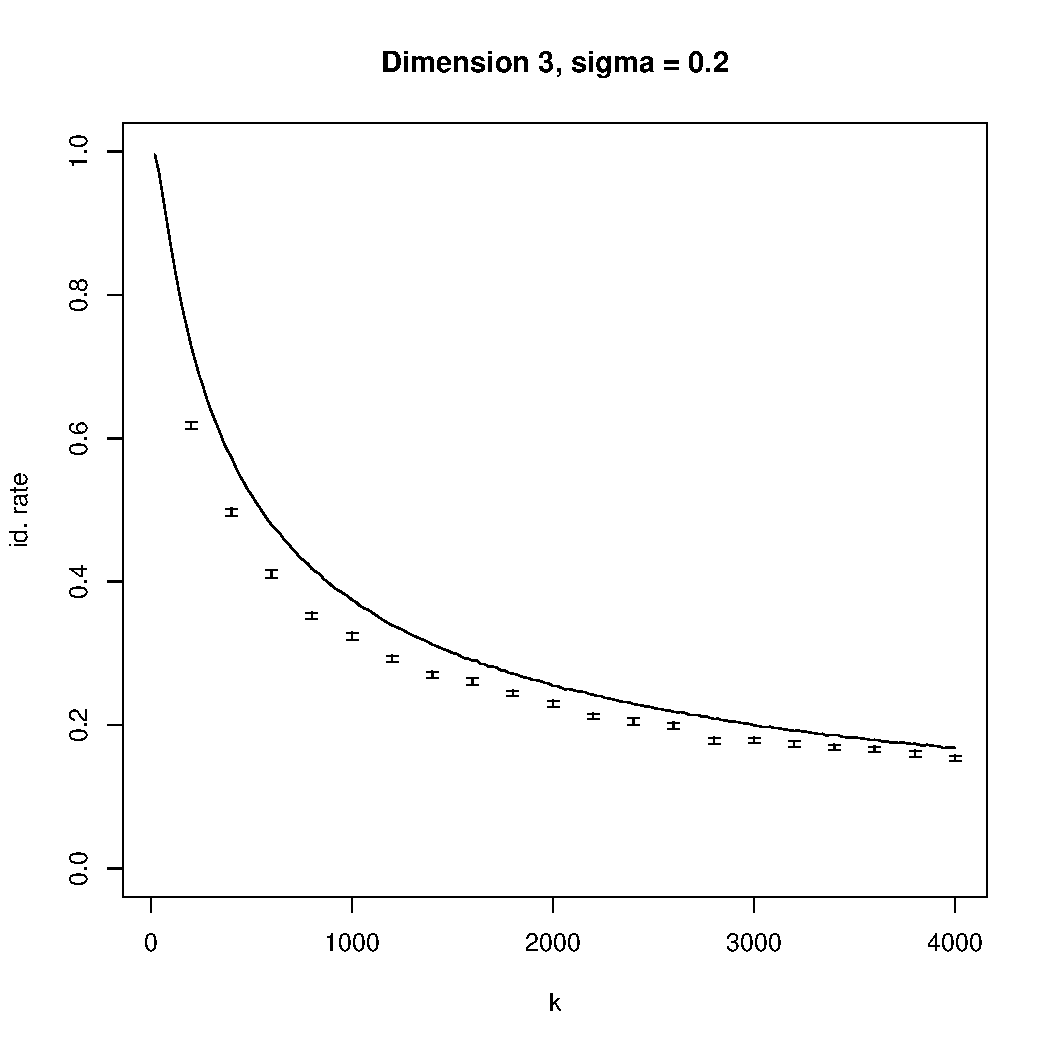
\includegraphics[scale = 0.6]{plot1_3.pdf}
\caption{Dimension 3, $\Sigma_\mu = I$,  $\sigma = 0.2$}
\end{figure}

\begin{figure}
\centering
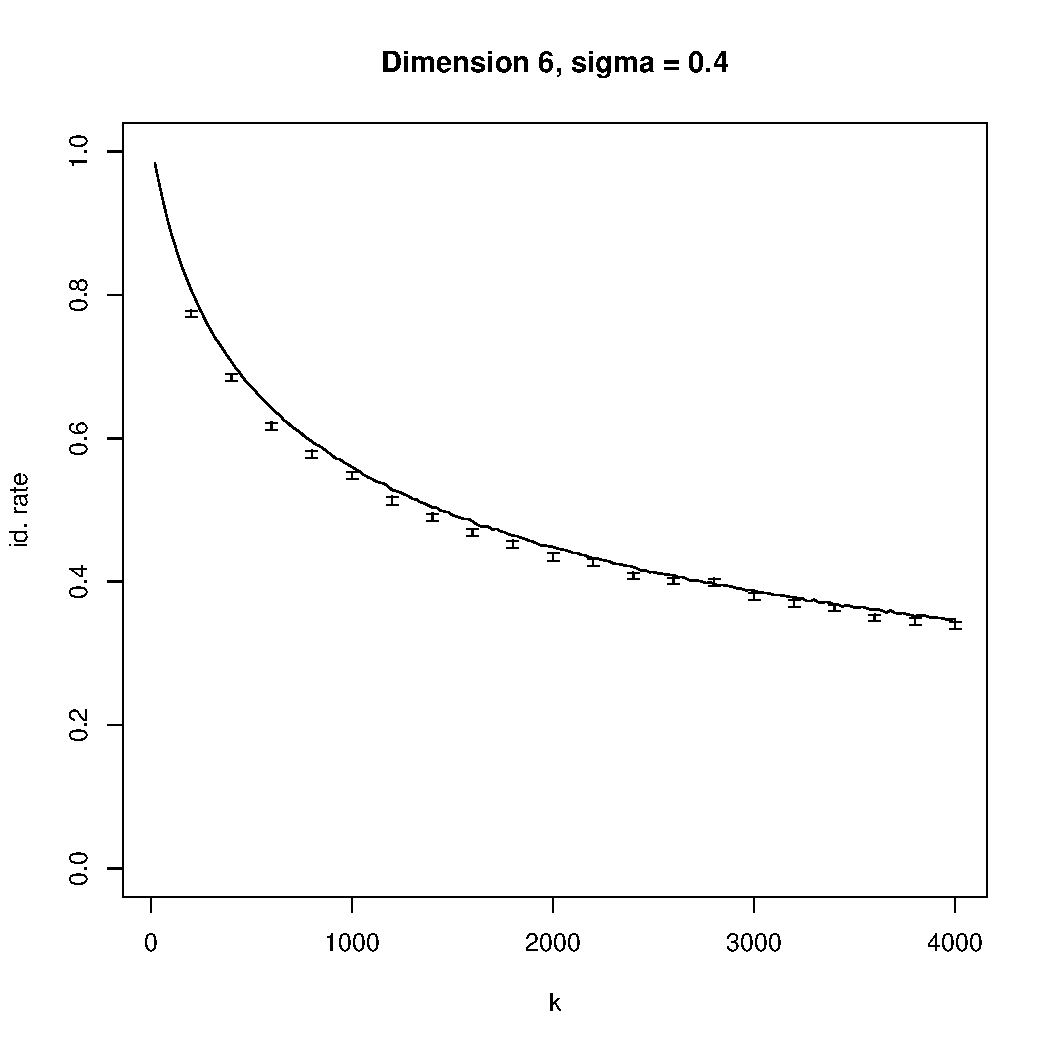
\includegraphics[scale = 0.6]{plot1_6.pdf}
\caption{Dimension 6, $\Sigma_\mu = I$, $\sigma = 0.4$}
\end{figure}

\begin{figure}
\centering
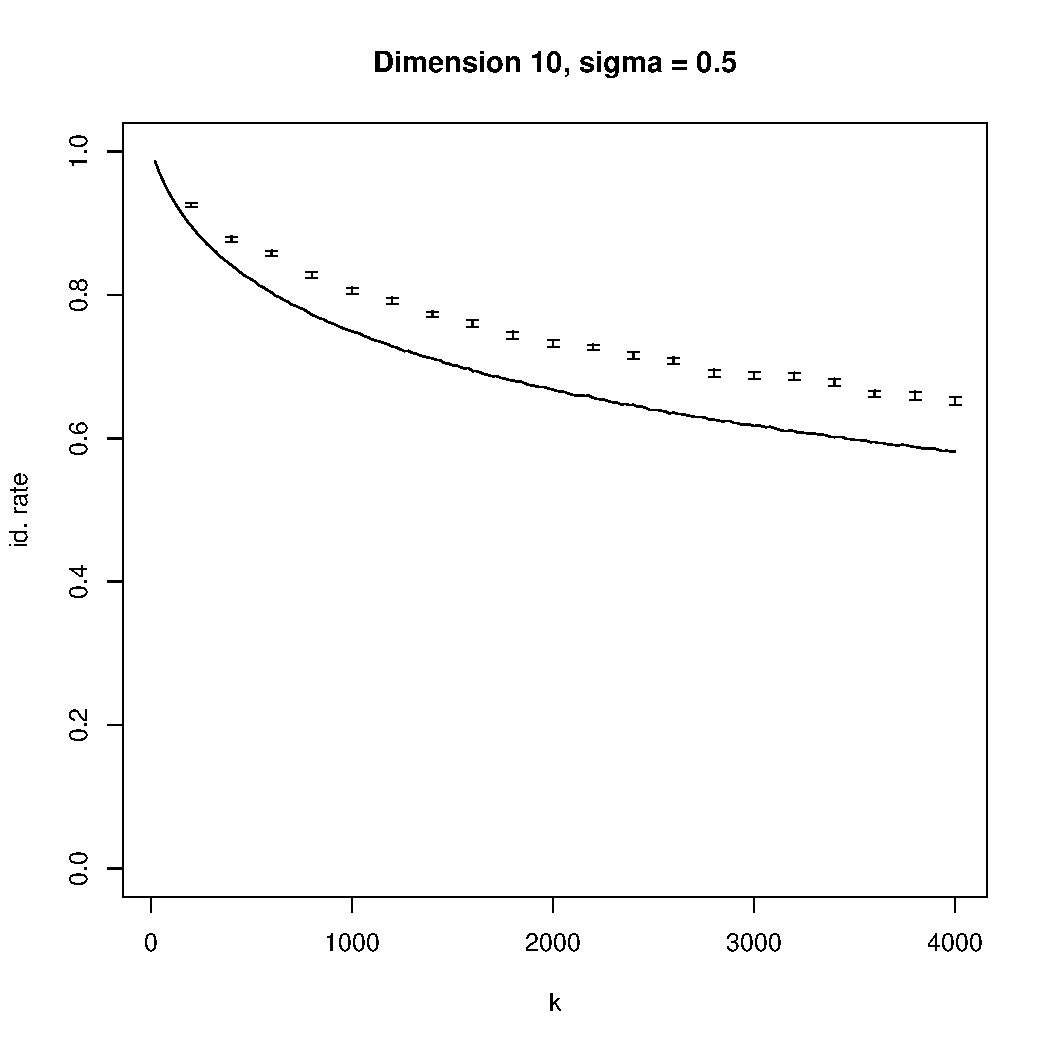
\includegraphics[scale = 0.6]{plot1_10.pdf}
\caption{Dimension 10, $\Sigma_\mu = I$, $\sigma = 0.5$}
\end{figure}

\end{document}
